% Pursuing Stacks (cotes 134-2 to 134-8): archive cote 134-3, site page 80 (PDF page 81), typescript page 80.
% typescript. Draft compared: ps2.tex:4144-4223.
% AI-transcribed by Claude Opus 5.5 (claude-opus-5-5, adaptive thinking, effort high), Message Batches API, batch ps1 (msgbatch_01Rv5hCaNTtUt4JHx1yqoHPL), 2026-11-12; image review recorded in records/CHECK_DECISIONS_134_3_4.tsv.
\scanpage{134-3/80}
\mspage{(80)}

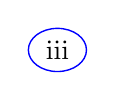
\begin{tikzpicture}[baseline=(n.base)]\node[inner sep=0pt] (n) {iii};\draw[color=blue,line width=.5pt] (n.center) ellipse [x radius=1.05em,y radius=.78em];\end{tikzpicture} As in (ii), but moreover the adjunction morphism in $W_A^{\hand{-1}}A^{\hand{\wedge}}$ for
the pair of quasi-inverse equivalences \inserted[typed]{(5)}, being \hand{likewise deduced from }\inserted{(4).}
(iv) For any C in (Cat), (3) is a weak equivalence.
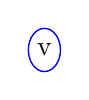
\begin{tikzpicture}[baseline=(n.base)]\node[inner sep=0pt] (n) {v};\draw[color=blue,line width=.5pt] (n.center) ellipse [x radius=.58em,y radius=.78em];\end{tikzpicture} Same as (iv), with C restricted to having a final element, i.e.
for any such C, $j_Ai_A(C) = A_{/j_A(C)}$ is a\over{\unsure{s}}{s}pheric.
(vi) For any F in $A^{\hand{\wedge}}$, (4) is a weak equivalence, moreover
\[ W_{(Cat)} = j_A^{-1}(W_A) \qquad , \]
i.e. a \xout{functor} map $f\colon C' \hand{\to} C$ in (Cat) is a \xout{quasi} \inserted[typed]{weak} equivalence,
iff $j_A(f)$ is a \xout{quasi} \inserted[typed]{weak} equivalence in $A^{\hand{\wedge}}$ - which means, by defi-%
n\over[typed]{\illegible{1}}{i}tion (more or less) that $i_Aj_A(f)$ is a \xout{quasi} \inserted[typed]{weak} equivalence.
(vii) T\over{h}{h}e functor
(6) \[ i_Aj_A \; : \; (Cat) \hand{\longrightarrow} (Cat) \quad , \quad C \hand{\mapsto} A_{/j_A(C)} \, , \]
transforms \xout{quasi} \inserted[typed]{weak} equivalences into \xout{quasi} \inserted[typed]{weak} equivalences , i.e.
gives rise to a functor (Hot)$\hand{\to}$(Hot), and moreover \deleted{A is} \hand{the}
\deleted{aspheric.} \hand{latter respects final object (i.e. A is aspheric).}
(viii) Same as (vii), but restricting to \xout{quax} weak equivalences of the
type $C \hand{\to} \over[typed]{e}{e}$, where C has a final element and e is the final
object in (Cat) (the one-point category)\hand{, plus asphericity of A.}

The trivial implications between all these conditions can be summari\xout{z}
zed in the diagram
% Hand-drawn arrows are marked blue; typed objects remain plain.
\diagram{\begin{tikzcd}[row sep=small, arrows=Rightarrow]
(iii) \ar[r,Leftrightarrow,color=blue] \ar[d,color=blue] \& (vi) \ar[r,color=blue] \& (vii) \ar[r,color=blue] \& (viii) \ar[dl,color=blue] \\
(ii) \ar[r,color=blue] \ar[d,color=blue] \& (iv) \ar[r,color=blue] \& (v) \& \\
(i) \& , \& \&
\end{tikzcd}}
the only \inserted[typed]{slightly} less obvious implication here is (viii)\hand{$\Rightarrow$}(v), which is seen
by looking at the commutative square deduced from $C \hand{\to} e$ (C in (Cat) as in
(v)\xout{\unsure{;}} namely with final element) by applying (3)
\diagram{\begin{tikzcd}
i_Aj_A(C) \ar[r,color=blue] \ar[d,color=blue] \& C \ar[d,color=blue] \\
A{=}i_Aj_A(e) \ar[r,color=blue] \& e
\end{tikzcd} \quad ,}
by assumption the vertical arrows are weak equivalences, and so is $A \hand{\to} e$
(because A is supposed to be aspheric), therefore the same holds for the
fourth arrow left. On the other hand an easy asphericity argument
showed us \inserted{[\unsure{\S}.30]} that (v) \hand{$\Longrightarrow$}(iii), hence all conditions (ii) to (viii) are
equivalent, and they are equivalent to the stronger form of (iv), \xout{that}
say (iv'), \over[typed]{d}{s}\over[typed]{a}{a}ying that (3) is \uline{aspheric} for any C in (Cat). T\over{h}{h}e only
equivalence which is not quite clear yet is that (i) implies the other
conditions\unsure{\over{,}{.}} \deleted{under the formally weakest form (v) let's say.} B\over{u}{u}t it is so
